\documentclass[]{article}

\usepackage{listings}	
\usepackage{float}
\usepackage{graphicx}

\usepackage{titling}
\newcommand{\subtitle}[1]{%
  \posttitle{%
    \par\end{center}
    \begin{center}\large#1\end{center}
    \vskip0.5em}%
}

\begin{document}

\title{Lab 2: Floating Point Conversion}
\subtitle{CS M152A}
\author{Aman Agarwal \& Lowell Bander}

\maketitle
\tableofcontents \newpage

\section{Introduction}

A linear encoding of bits can be interpreted many different ways, for example as unsigned integers, signed integers in 2's complement, and even as floating point values. In this lab we learn how to convert bits in 2's complement to a simple floating point representation.

The input is a 12-bit 2's complement signed integer. The output is an 8-bit floating point value. The 8 bits are split up so that the 1st represents the sign, the next 3, the exponenent, and the last 4, the significand.

\begin{displaymath}
V = (-1)^S \times F \times 2^E
\end{displaymath}

Because 2's complement signed integers don't necessarily map directly to floating point values, we must map these to their closest floating point value through the process of rounding. By using the simple rounding rule provided, we are able to get the closest floating point value for each integer. Without rounding, we only get accurate results for about half of the inputs (those that would round down).

\section{Design Description}

\subsection{High Level Design}
\label{subsec:highlevel}

To convert a value from its representation as a 12 bit two's-complement number to an 8 bit floating point number, we used 3 main modules. The first of which converted the input from a two's complement representation to a sign-magnitude representation. The second counts the number of leading zeros to determine the value of the exponent, and extracts the lower bits for use in determining the exponent. The third and final module handles the edge cases, such as rounding the significand and handling overflow.\\

Before we began implementing the converter in Verilog, we first drew up a schematic in Logisim, as pictured in Figure~\ref{fig:logisim}.\\

\begin{figure}[H]
\centering
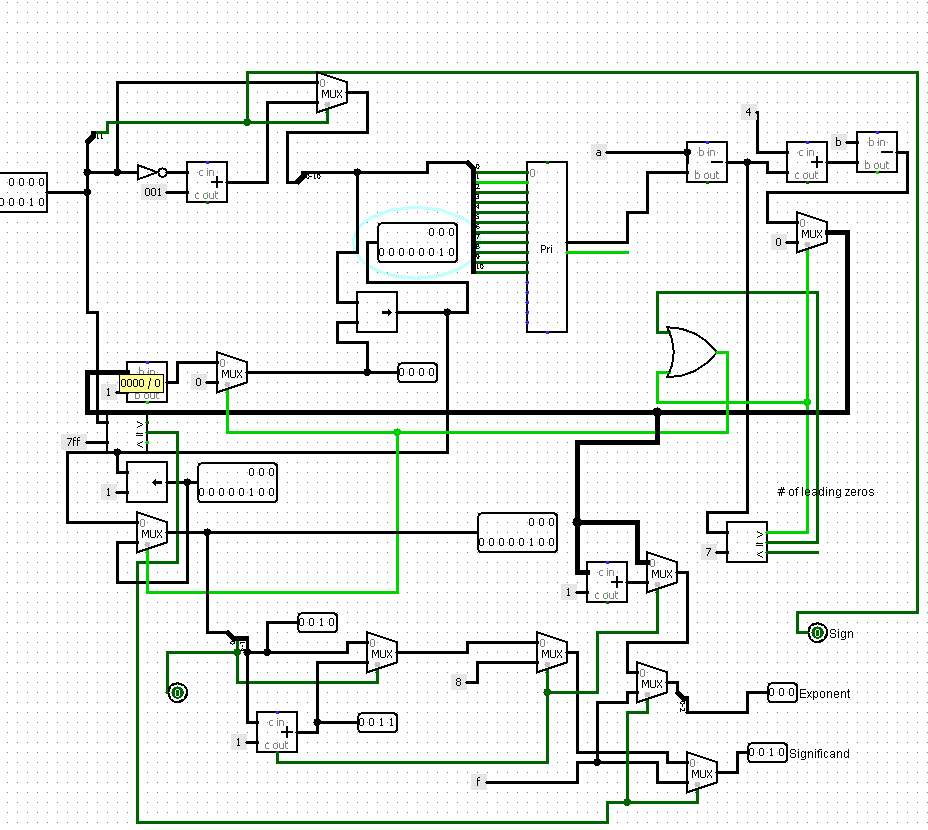
\includegraphics[width=11cm]{logisim.PNG}
\caption{A schematic for the converted drawn using Logisim. Input is delivered to the system in the upper-left, and output is found in the lower-right.}
\label{fig:logisim}
\end{figure}

\subsection{Low Level Implementation}

The source code displayed below is an a excerpt from our main module, \texttt{fpcvt.v}. The 3 modules described in subsection~\ref{subsec:highlevel} above are show here with the following mapping: The first module described above is composed of the first module shown below, which takes as input a 12 bit two's complement integer, and outputs an 8 bit sign-magnitude integer.\\

The next two modules have the same semantics as the second modules described above. The first modules, \texttt{leadingZeroesCount}, takes as input the magnitude of the input number, and outputs the number of leading zeros, for use later in determining the exponent. The following module, \texttt{extractSignificandAndRoundBit}, takes as input the magnitude of the input value and the number of leading zeros, and returns the 4-bit significand and the fifth bit used for rounding.\\

The final two modules below implement the 3rd module described above in subsection~\ref{subsec:highlevel}. The first of which, \texttt{roundValueIfRound}, takes as input the intermediate significand produced by the \texttt{extractSignificand\-AndRoundBit} module, as well as the fifth bit outputted by the the same module. The outputs of this modules are the rounded significand, if this was necessary, and a bit indicating whether overflow results from this rounding. The final module, \texttt{handleOverflow}, handles possible overflow by right shifting the significand and incrementing the exponent to account for this increment.

\begin{lstlisting}[frame=single, language=verilog, caption= Excerpt from main \texttt{fpcvt.v} module.]
twosComplementToSignMagnitude ttsm(.I(D), .S(S), .M(mag));
    
leadingZeroesCount lzc(.I(mag), .O(zeroCount));
    
extractSignicifandAndRoundBit esr(.I(mag), 
.zeros(zeroCount), .significand(tempF), .round(round));

roundValueIfRound rvir(.I(tempF), .roundedVal(rv), 
.Round(round), .overflow(overflow));

handleOverflow ho(.I(D), .roundedVal(rv), .significand(F), 
.oldE(tempE), .exponent(E), .overflow(overflow));
\end{lstlisting}

\section{Simulation Documentation}
\section{Conclusion}
For most cases we tested, our Logisim schematic outputted the expected values. It only failed for a few edge cases, which we remedied with hack-y fixes that modified our result for the very specific extremes encountered during floating point conversion. However, our conversion from Logisim to Verilog was imperfect, and we often had logic errors as a result of forgetting to implement parts of modules in Verilog which we had implemented in Logisim.\\

We often stumbled due to misunderstandings of Verilog, such as when to use \texttt{wire} instead of \texttt{reg}. We also made the mistake of writing all of our code before testing it, creating our textbench \texttt{tb.v} at the very end.

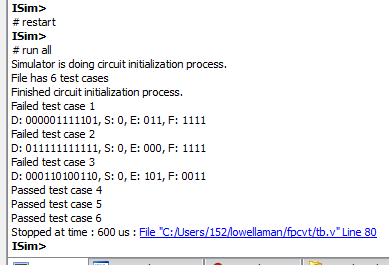
\includegraphics[width=10cm]{output.PNG}

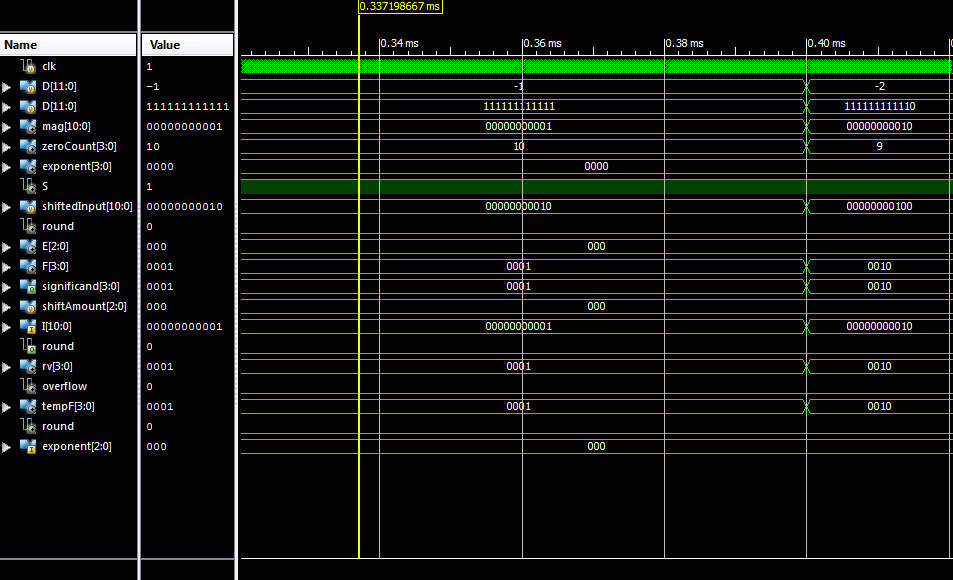
\includegraphics[width=10cm]{waveform.PNG}

\lstinputlisting[language=Verilog, firstline=1, lastline=2]{fpcvt.v}

\lstinputlisting[language=Verilog, firstline=25, lastline=26]{tb.v}

\end{document}

